\documentclass{standalone}
\usepackage{tikz}
\usetikzlibrary{patterns, positioning}
\usepackage[sfdefault]{ClearSans} %% option 'sfdefault' activates Clear Sans as the default text font
\usepackage[T1]{fontenc}

\begin{document}
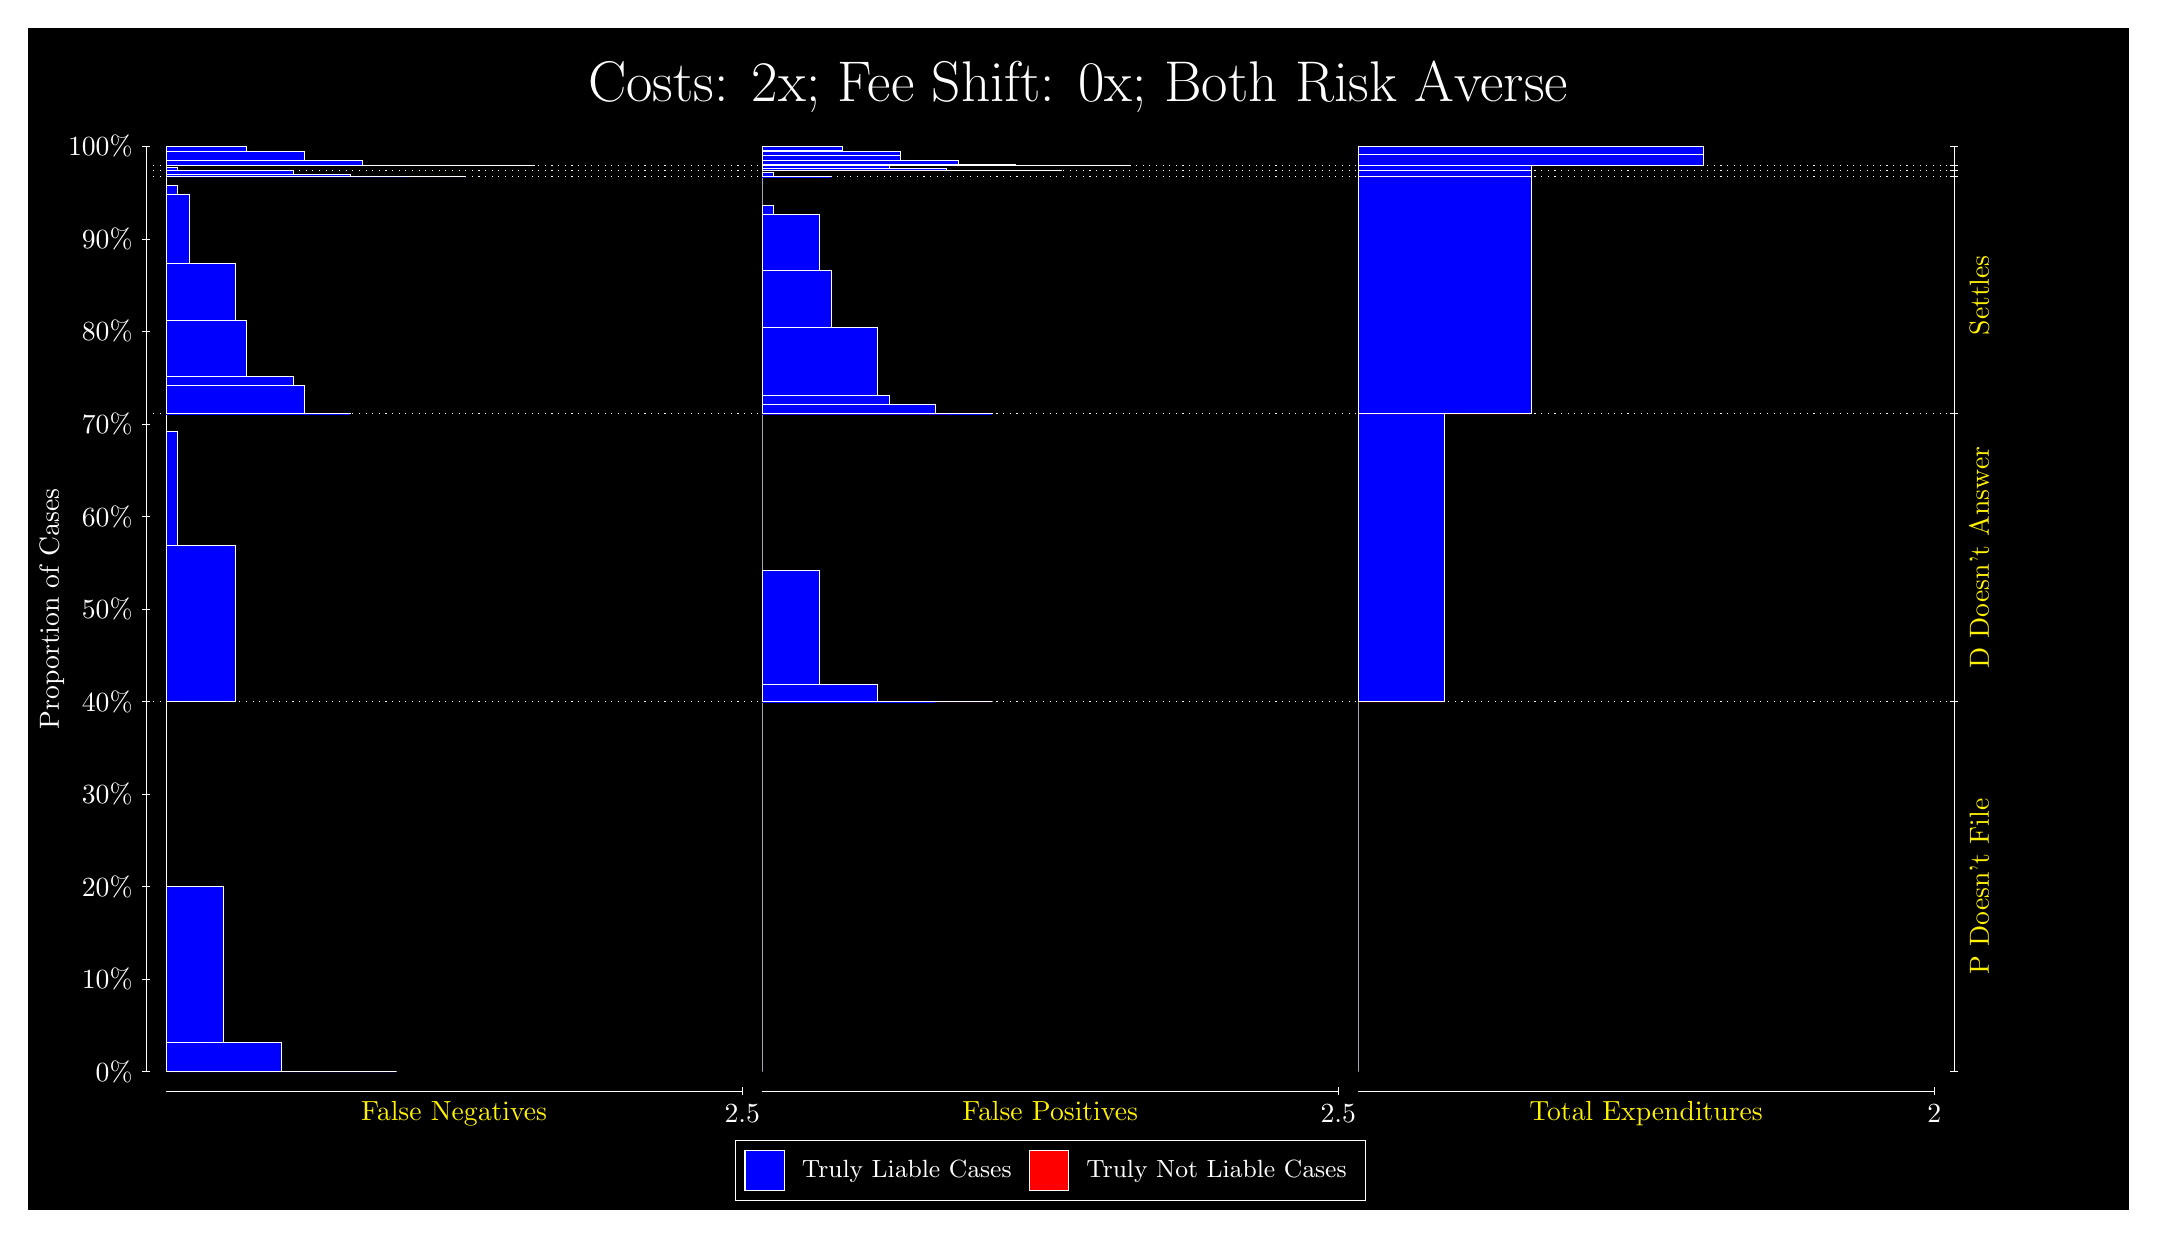
\begin{tikzpicture}
\draw[fill=black] (0,0) rectangle (26.667,15);
\draw[text=white] (0,13.5) rectangle (26.667,15) node[midway] {\huge Costs: 2x; Fee Shift: 0x; Both Risk Averse};
\draw[white, very thin] (1.5,1.75) -- (1.5,13.5);
\node[rotate=90, text=white, anchor=center] at (0.3, 7.625) {Proportion of Cases};
\draw[white, very thin] (1.45,1.75) -- (1.55,1.75);
\node[text=white, anchor=east] at (1.45, 1.75) {0\%};
\draw[white, very thin] (1.45,2.925) -- (1.55,2.925);
\node[text=white, anchor=east] at (1.45, 2.925) {10\%};
\draw[white, very thin] (1.45,4.1) -- (1.55,4.1);
\node[text=white, anchor=east] at (1.45, 4.1) {20\%};
\draw[white, very thin] (1.45,5.275) -- (1.55,5.275);
\node[text=white, anchor=east] at (1.45, 5.275) {30\%};
\draw[white, very thin] (1.45,6.45) -- (1.55,6.45);
\node[text=white, anchor=east] at (1.45, 6.45) {40\%};
\draw[white, very thin] (1.45,7.625) -- (1.55,7.625);
\node[text=white, anchor=east] at (1.45, 7.625) {50\%};
\draw[white, very thin] (1.45,8.8) -- (1.55,8.8);
\node[text=white, anchor=east] at (1.45, 8.8) {60\%};
\draw[white, very thin] (1.45,9.975) -- (1.55,9.975);
\node[text=white, anchor=east] at (1.45, 9.975) {70\%};
\draw[white, very thin] (1.45,11.15) -- (1.55,11.15);
\node[text=white, anchor=east] at (1.45, 11.15) {80\%};
\draw[white, very thin] (1.45,12.325) -- (1.55,12.325);
\node[text=white, anchor=east] at (1.45, 12.325) {90\%};
\draw[white, very thin] (1.45,13.5) -- (1.55,13.5);
\node[text=white, anchor=east] at (1.45, 13.5) {100\%};

\draw[white, very thin] (24.457,1.75) -- (24.457,13.5);
\draw[white, very thin] (24.407,1.75) -- (24.507,1.75);
\node[anchor=west] at (24.407, 1.75) {};
\draw[white, very thin] (24.407,6.4489) -- (24.507,6.4489);
\node[anchor=west] at (24.407, 6.4489) {};
\draw[white, very thin] (24.407,10.104) -- (24.507,10.104);
\node[anchor=west] at (24.407, 10.104) {};
\draw[white, very thin] (24.407,13.115) -- (24.507,13.115);
\node[anchor=west] at (24.407, 13.115) {};
\draw[white, very thin] (24.407,13.196) -- (24.507,13.196);
\node[anchor=west] at (24.407, 13.196) {};
\draw[white, very thin] (24.407,13.261) -- (24.507,13.261);
\node[anchor=west] at (24.407, 13.261) {};
\draw[white, very thin] (24.407,13.5) -- (24.507,13.5);
\node[anchor=west] at (24.407, 13.5) {};

\draw[white, very thin, fill=blue] (1.75,1.75) rectangle (4.6775,1.75);
\draw[white, very thin, fill=blue] (1.75,1.75) rectangle (3.9457,1.7532);
\draw[white, very thin, fill=blue] (1.75,1.7532) rectangle (3.2138,2.126);
\draw[white, very thin, fill=blue] (1.75,2.126) rectangle (2.4819,4.1027);
\draw[white, very thin, fill=red] (1.75,4.1027) rectangle (1.75,4.1027);
\draw[white, very thin, fill=blue] (1.75,4.1027) rectangle (1.75,6.4489);
\draw[white, very thin, fill=blue] (1.75,6.4489) rectangle (2.6283,8.4332);
\draw[white, very thin, fill=blue] (1.75,8.4332) rectangle (1.8964,9.8836);
\draw[white, very thin, fill=red] (1.75,9.8836) rectangle (1.75,9.8836);
\draw[white, very thin, fill=blue] (1.75,9.8836) rectangle (1.75,10.104);
\draw[white, very thin, fill=blue] (1.75,10.104) rectangle (4.092,10.105);
\draw[white, very thin, fill=blue] (1.75,10.105) rectangle (3.5065,10.468);
\draw[white, very thin, fill=blue] (1.75,10.468) rectangle (3.3602,10.582);
\draw[white, very thin, fill=blue] (1.75,10.582) rectangle (2.7746,11.291);
\draw[white, very thin, fill=blue] (1.75,11.291) rectangle (2.6283,12.017);
\draw[white, very thin, fill=blue] (1.75,12.017) rectangle (2.0428,12.888);
\draw[white, very thin, fill=blue] (1.75,12.888) rectangle (1.8964,13.001);
\draw[white, very thin, fill=red] (1.75,13.001) rectangle (1.75,13.001);
\draw[white, very thin, fill=blue] (1.75,13.001) rectangle (1.75,13.115);
\draw[white, very thin, fill=blue] (1.75,13.115) rectangle (5.5558,13.115);
\draw[white, very thin, fill=blue] (1.75,13.115) rectangle (4.8239,13.115);
\draw[white, very thin, fill=blue] (1.75,13.115) rectangle (4.092,13.145);
\draw[white, very thin, fill=blue] (1.75,13.145) rectangle (3.3602,13.195);
\draw[white, very thin, fill=blue] (1.75,13.195) rectangle (2.6283,13.196);
\draw[white, very thin, fill=red] (1.75,13.196) rectangle (1.75,13.196);
\draw[white, very thin, fill=blue] (1.75,13.196) rectangle (2.6283,13.197);
\draw[white, very thin, fill=blue] (1.75,13.197) rectangle (1.8964,13.237);
\draw[white, very thin, fill=red] (1.75,13.237) rectangle (1.75,13.237);
\draw[white, very thin, fill=blue] (1.75,13.237) rectangle (1.75,13.261);
\draw[white, very thin, fill=blue] (1.75,13.261) rectangle (6.4341,13.261);
\draw[white, very thin, fill=blue] (1.75,13.261) rectangle (5.7022,13.261);
\draw[white, very thin, fill=blue] (1.75,13.261) rectangle (4.9703,13.264);
\draw[white, very thin, fill=blue] (1.75,13.264) rectangle (4.2384,13.319);
\draw[white, very thin, fill=blue] (1.75,13.319) rectangle (3.5065,13.44);
\draw[white, very thin, fill=blue] (1.75,13.44) rectangle (2.7746,13.495);
\draw[white, very thin, fill=blue] (1.75,13.495) rectangle (2.0428,13.5);
\draw[white, very thin, fill=red] (1.75,13.5) rectangle (1.75,13.5);
\draw[white, very thin, fill=blue] (1.75,13.5) rectangle (1.75,13.5);
\draw[white, very thin, fill=red] (9.3189,1.75) rectangle (9.3189,1.75);
\draw[white, very thin, fill=blue] (9.3189,1.75) rectangle (9.3189,6.4489);
\draw[white, very thin, fill=red] (9.3189,6.4489) rectangle (12.246,6.4489);
\draw[white, very thin, fill=blue] (9.3189,6.4489) rectangle (12.246,6.4489);
\draw[white, very thin, fill=blue] (9.3189,6.4489) rectangle (11.515,6.4493);
\draw[white, very thin, fill=blue] (9.3189,6.4493) rectangle (10.783,6.6698);
\draw[white, very thin, fill=blue] (9.3189,6.6698) rectangle (10.051,8.1202);
\draw[white, very thin, fill=blue] (9.3189,8.1202) rectangle (9.3189,10.104);
\draw[white, very thin, fill=red] (9.3189,10.104) rectangle (12.246,10.104);
\draw[white, very thin, fill=blue] (9.3189,10.104) rectangle (12.246,10.105);
\draw[white, very thin, fill=red] (9.3189,10.105) rectangle (11.661,10.105);
\draw[white, very thin, fill=blue] (9.3189,10.105) rectangle (11.661,10.105);
\draw[white, very thin, fill=blue] (9.3189,10.105) rectangle (11.515,10.218);
\draw[white, very thin, fill=blue] (9.3189,10.218) rectangle (10.929,10.332);
\draw[white, very thin, fill=blue] (9.3189,10.332) rectangle (10.783,11.202);
\draw[white, very thin, fill=blue] (9.3189,11.202) rectangle (10.197,11.928);
\draw[white, very thin, fill=blue] (9.3189,11.928) rectangle (10.051,12.638);
\draw[white, very thin, fill=blue] (9.3189,12.638) rectangle (9.4652,12.751);
\draw[white, very thin, fill=blue] (9.3189,12.751) rectangle (9.3189,13.115);
\draw[white, very thin, fill=red] (9.3189,13.115) rectangle (10.197,13.115);
\draw[white, very thin, fill=blue] (9.3189,13.115) rectangle (10.197,13.116);
\draw[white, very thin, fill=blue] (9.3189,13.116) rectangle (9.4652,13.166);
\draw[white, very thin, fill=blue] (9.3189,13.166) rectangle (9.3189,13.196);
\draw[white, very thin, fill=red] (9.3189,13.196) rectangle (13.125,13.196);
\draw[white, very thin, fill=blue] (9.3189,13.196) rectangle (13.125,13.196);
\draw[white, very thin, fill=blue] (9.3189,13.196) rectangle (12.393,13.196);
\draw[white, very thin, fill=blue] (9.3189,13.196) rectangle (11.661,13.22);
\draw[white, very thin, fill=blue] (9.3189,13.22) rectangle (10.929,13.26);
\draw[white, very thin, fill=blue] (9.3189,13.26) rectangle (10.197,13.261);
\draw[white, very thin, fill=red] (9.3189,13.261) rectangle (14.003,13.261);
\draw[white, very thin, fill=blue] (9.3189,13.261) rectangle (14.003,13.261);
\draw[white, very thin, fill=red] (9.3189,13.261) rectangle (13.271,13.261);
\draw[white, very thin, fill=blue] (9.3189,13.261) rectangle (13.271,13.261);
\draw[white, very thin, fill=red] (9.3189,13.261) rectangle (12.539,13.261);
\draw[white, very thin, fill=blue] (9.3189,13.261) rectangle (12.539,13.266);
\draw[white, very thin, fill=blue] (9.3189,13.266) rectangle (11.807,13.321);
\draw[white, very thin, fill=red] (9.3189,13.321) rectangle (11.807,13.321);
\draw[white, very thin, fill=blue] (9.3189,13.321) rectangle (11.807,13.321);
\draw[white, very thin, fill=blue] (9.3189,13.321) rectangle (11.075,13.391);
\draw[white, very thin, fill=red] (9.3189,13.391) rectangle (11.075,13.391);
\draw[white, very thin, fill=blue] (9.3189,13.391) rectangle (11.075,13.442);
\draw[white, very thin, fill=blue] (9.3189,13.442) rectangle (10.344,13.45);
\draw[white, very thin, fill=blue] (9.3189,13.45) rectangle (10.344,13.497);
\draw[white, very thin, fill=blue] (9.3189,13.497) rectangle (9.6116,13.497);
\draw[white, very thin, fill=blue] (9.3189,13.497) rectangle (9.6116,13.5);
\draw[white, very thin, fill=blue] (9.3189,13.5) rectangle (9.3189,13.5);
\draw[white, very thin, fill=red] (16.888,1.75) rectangle (16.888,1.75);
\draw[white, very thin, fill=blue] (16.888,1.75) rectangle (16.888,6.4489);
\draw[white, very thin, fill=red] (16.888,6.4489) rectangle (17.986,6.4489);
\draw[white, very thin, fill=blue] (16.888,6.4489) rectangle (17.986,10.104);
\draw[white, very thin, fill=red] (16.888,10.104) rectangle (19.083,10.104);
\draw[white, very thin, fill=blue] (16.888,10.104) rectangle (19.083,13.115);
\draw[white, very thin, fill=red] (16.888,13.115) rectangle (19.083,13.115);
\draw[white, very thin, fill=blue] (16.888,13.115) rectangle (19.083,13.196);
\draw[white, very thin, fill=red] (16.888,13.196) rectangle (19.083,13.196);
\draw[white, very thin, fill=blue] (16.888,13.196) rectangle (19.083,13.261);
\draw[white, very thin, fill=red] (16.888,13.261) rectangle (21.279,13.261);
\draw[white, very thin, fill=blue] (16.888,13.261) rectangle (21.279,13.399);
\draw[white, very thin, fill=red] (16.888,13.399) rectangle (21.279,13.399);
\draw[white, very thin, fill=blue] (16.888,13.399) rectangle (21.279,13.5);
\draw[white, dotted] (1.5,6.4489) -- (24.457,6.4489);
\draw[white, dotted] (1.5,10.104) -- (24.457,10.104);
\draw[white, dotted] (1.5,13.115) -- (24.457,13.115);
\draw[white, dotted] (1.5,13.196) -- (24.457,13.196);
\draw[white, dotted] (1.5,13.261) -- (24.457,13.261);
\draw[white, very thin] (1.75,1.5) -- (9.0689,1.5);
\node[text=yellow, anchor=north] at (5.4094, 1.5) {False Negatives};
\draw[white, very thin] (9.0689,1.45) -- (9.0689,1.55);
\node[text=white, anchor=north] at (9.0689, 1.45) {2.5};

\draw[white, very thin] (9.3189,1.5) -- (16.638,1.5);
\node[text=yellow, anchor=north] at (12.978, 1.5) {False Positives};
\draw[white, very thin] (16.638,1.45) -- (16.638,1.55);
\node[text=white, anchor=north] at (16.638, 1.45) {2.5};

\draw[white, very thin] (16.888,1.5) -- (24.207,1.5);
\node[text=yellow, anchor=north] at (20.547, 1.5) {Total Expenditures};
\draw[white, very thin] (24.207,1.45) -- (24.207,1.55);
\node[text=white, anchor=north] at (24.207, 1.45) {2};

\node[text=yellow, centered, rotate=90] at (24.777, 4.0995) {P Doesn't File};
\node[text=yellow, centered, rotate=90] at (24.777, 8.2767) {D Doesn't Answer};
\node[text=yellow, centered, rotate=90] at (24.777, 11.61) {Settles};




\draw (12.978300999999998,1.5) node[draw=none] (baseCoordinate) {};
\begin{scope}[align=center]
        \matrix[scale=0.5, draw=white, below=0.5cm of baseCoordinate, nodes={draw}, column sep=0.1cm]{
            \node[rectangle, draw, minimum width=0.5cm, minimum height=0.5cm, fill=blue] {}; &
            \node[draw=none, font=\small, text=white] (B) {Truly Liable Cases}; &
            \node[rectangle, draw, minimum width=0.5cm, minimum height=0.5cm, fill=red] {}; &
            \node[draw=none, font=\small, text=white] (B) {Truly Not Liable Cases}; \\
            };
\end{scope}

\end{tikzpicture}
\end{document}